\documentclass[11pt]{article}


\usepackage{geometry}
\usepackage{subcaption} 
\geometry{letterpaper}


\usepackage{doc}
\usepackage{cite}
\usepackage[margin=1cm]{caption}

\usepackage{url}


\usepackage{graphicx}
\usepackage{epstopdf}
\DeclareGraphicsRule{.tif}{png}{.png}{`convert #1 `dirname #1`/`basename #1 .tif`.png}


\title{A ``Dream'' Interface Design}
\author{Rachel Rivera}
\date{November 25, 2014}


\begin{document}


\maketitle


\begin{abstract}
This investigation presents a ``dream'' user interface design for touch screen mobile devices. This design aims to tackle the usability issue of insufficient feedback as well as provide an interface that is user-friendly for individuals with visual impairments and individuals without visual impairments alike. Of the five prevalent usability metrics within the field of Interaction Design, the three metrics of learnability, efficiency, and errors were particularly significant in the creation and development of this interface design \cite{Nielsen:1993:UE:529793}.
\end{abstract}


\pagebreak
\tableofcontents



\pagebreak


\section{Introduction}
\label{Introduction}

Mobile devices are ubiquitous in contemporary society. The latest figures from the United Nations' telecommunications agency estimate that there are around 6.8 billion cell-phone subscriptions in the world \cite{UNTelecommunications	}. Thus, the investigation and development of usable interfaces for mobile devices is a significant research topic.

Many of these mobile devices today utilize touch screens instead of physical keyboards or buttons. This allows for a larger display without increasing the size of the device. Furthermore, touchscreen keyboards and buttons have the ability to change their layout based on user input and disappear when not needed. To compensate for the lack of tactile feedback provided by physical keys and buttons, touchscreen devices often include aural feedback in the form of audible clicks from a speaker. Haptic feedback in the form of device vibrations is often included as well.

Even with these alternate forms of feedback, the literature suggests that insufficient feedback is still a major usability issue with touchscreen mobile devices. \cite{Tinwala:2010:ETE:18	68914.1868972, Kane:2011:UGB:1978942.1979001, Hardy:2008:TIT:1409240.1409267, El-Glaly:2013:TTF:2460625.2460665, Buxton:1986:HID:22339.22386}. A study by Hussain Tinwala and Scott MacKenzie submits that the lack of physical keys requires heightened visual attention from the user, which diverts the user's concentration from the thoughts being expressed \cite{Tinwala:2010:ETE:18 68914.1868972}. The lack of physical keys not only diverts the attention of some users, but it also makes the device  almost entirely unusable for other users. A study from Virginia Polytechnic Institute and State University demonstrates how touchscreen mobile devices do not provide sufficient feedback for Individuals with Blindness or Severe Visual Impairment (IBSVI) since these users are only able to develop a spatial mental model for the interface or the screen through ``dead reckoning'' \cite{El-Glaly:2013:TTF:2460625.2460665}. 

Thus, the aim of this investigation is to propose a ``dream'' interface design that addresses this usability issue.


\section{System Description}
\label{System Description}

In this investigation, I present a ``dream'' interface design for touchscreen mobile devices that focuses on providing the user with as much as feedback as possible. This feedback is designed in a way that aims to be helpful for users with visual impairments and users without visual impairments alike. The design in its entirety was created with the usability metrics of learnability, efficiency, and error rate in mind.

My ``dream'' interface design incorporates functionality of a product that is currently being developed by Tactus Technology \cite{Tactus}. Tactus Technology, a company based in Fremont, California, creates real physical buttons that dynamically appear and disappear into a flat touch screen (see Figure~\ref{tactus1}). Small fluid channels are routed throughout the Tactile Layer and enable fluid to expand the top polymer layer to create the physical buttons \cite{Tactus}.

Although this technology from Tactus is extremely bleeding-edge, the prototypes have already received a fair amount of recognition as well as several awards \cite{CNN, I-Zone, PCMag, Wired}. Reviewers have articulated how the technology seems to be ``downright magical'' \cite{CNN}. Though the look and feel of Tatctus technology seems totally futuristic, the technology is already beginning to appear in consumer devices. In 2013, Touch Revolution, the largest-volume glass projected capacitive multi-touch screen manufacturer in the world, announced a partnership with Tactus Technology \cite{TactusAvailability}. The technologies from the two companies are being combined and manufactured into consumer devices today \cite{TactusAvailability}. Not only is this technology becoming more and more available, but it is becoming more customizable as well. Companies will soon be able to customize the panel for different types of buttons, say for example, the buttons on a TV remote \cite{CNN}.

\begin{figure}[ht]
\centering
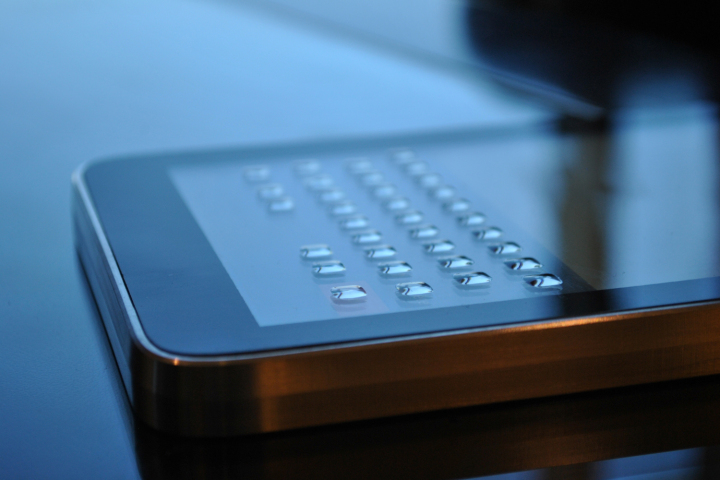
\includegraphics[width=4.5in]{tactus2.jpg} 
\caption{Tactus Technology keyboard}
\label{tactus1}
\end{figure}

My ``dream'' user interface design makes use of the varied tactile feedback that this technology from Tactus can provide.


\section{Top-Level Design}
The objective of this ``dream'' interface design is to make mobile touchscreen devices more usable for individuals with visual impairments and individuals without visual impairments alike. The three main features of the design used to attempt to accomplish this goal are the optional physical grid, the ``intelligent'' tactile buttons, and the auditory feedback. 


\subsection{Optional Physical Grid}
The design incorporates Tactus technology in order to provide an optional tactile grid for the device (see Figure~\ref{wireframe-grid}). The grid layout would consist of a set of very thin, three-dimensional horizontal and vertical lines. If the grid is enabled by the user, the set of horizontal and vertical lines appear on the screen. If the grid is disabled by the user, the lines recede. The horizontal and vertical lines are arranged with equal space between each line. The main purpose of this grid is to help IBSVI formulate a mental reference for location awareness. The fact that the grid can easily be disabled makes this feature unobtrusive for users who do not find benefit from it.


\begin{figure}[ht]
\centering
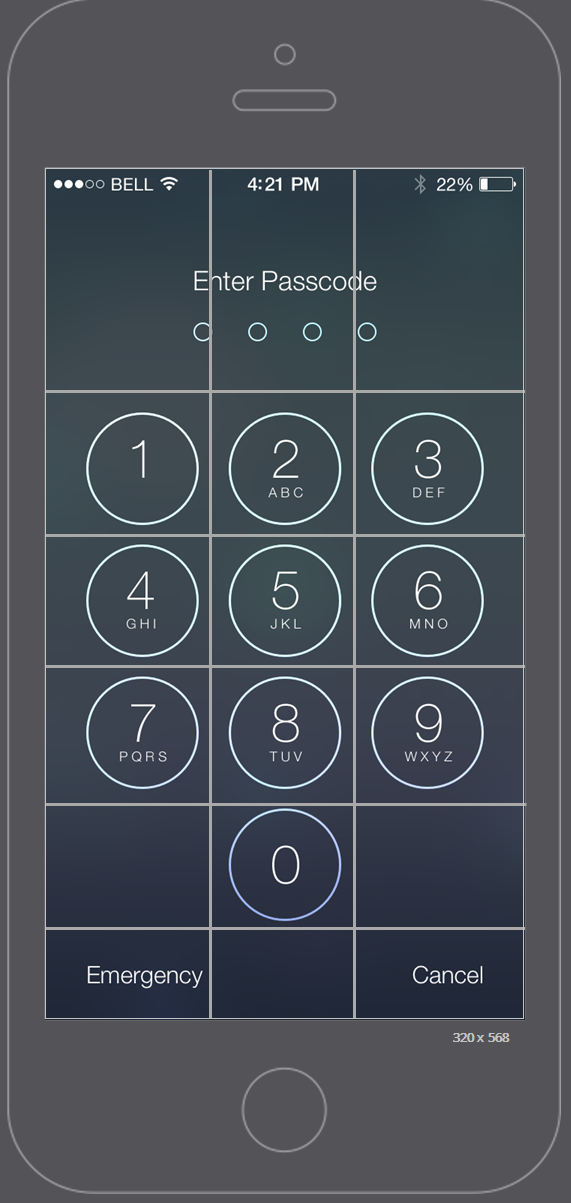
\includegraphics[width=2in]{wireframe-grid.png} 
\caption{A simple wireframe demonstrating the concept of the grid layout. Each line within the screen would actually be a physical line that appears on the screen with the use of Tactus's microfluidic technology.}
\label{wireframe-grid}
\end{figure}

\subsection{``Intelligent'' Tactile Buttons}
The design also includes tactile buttons that rise up and recede as needed (see Figure~\ref{buttons}). This aspect of the design would also be made possible with the use of technology from Tactus. Ideally, the mobile device would be ``intelligent'' about which buttons rose up on the flat screen depending on input from the user.
 
\begin{figure}[ht]
\centering
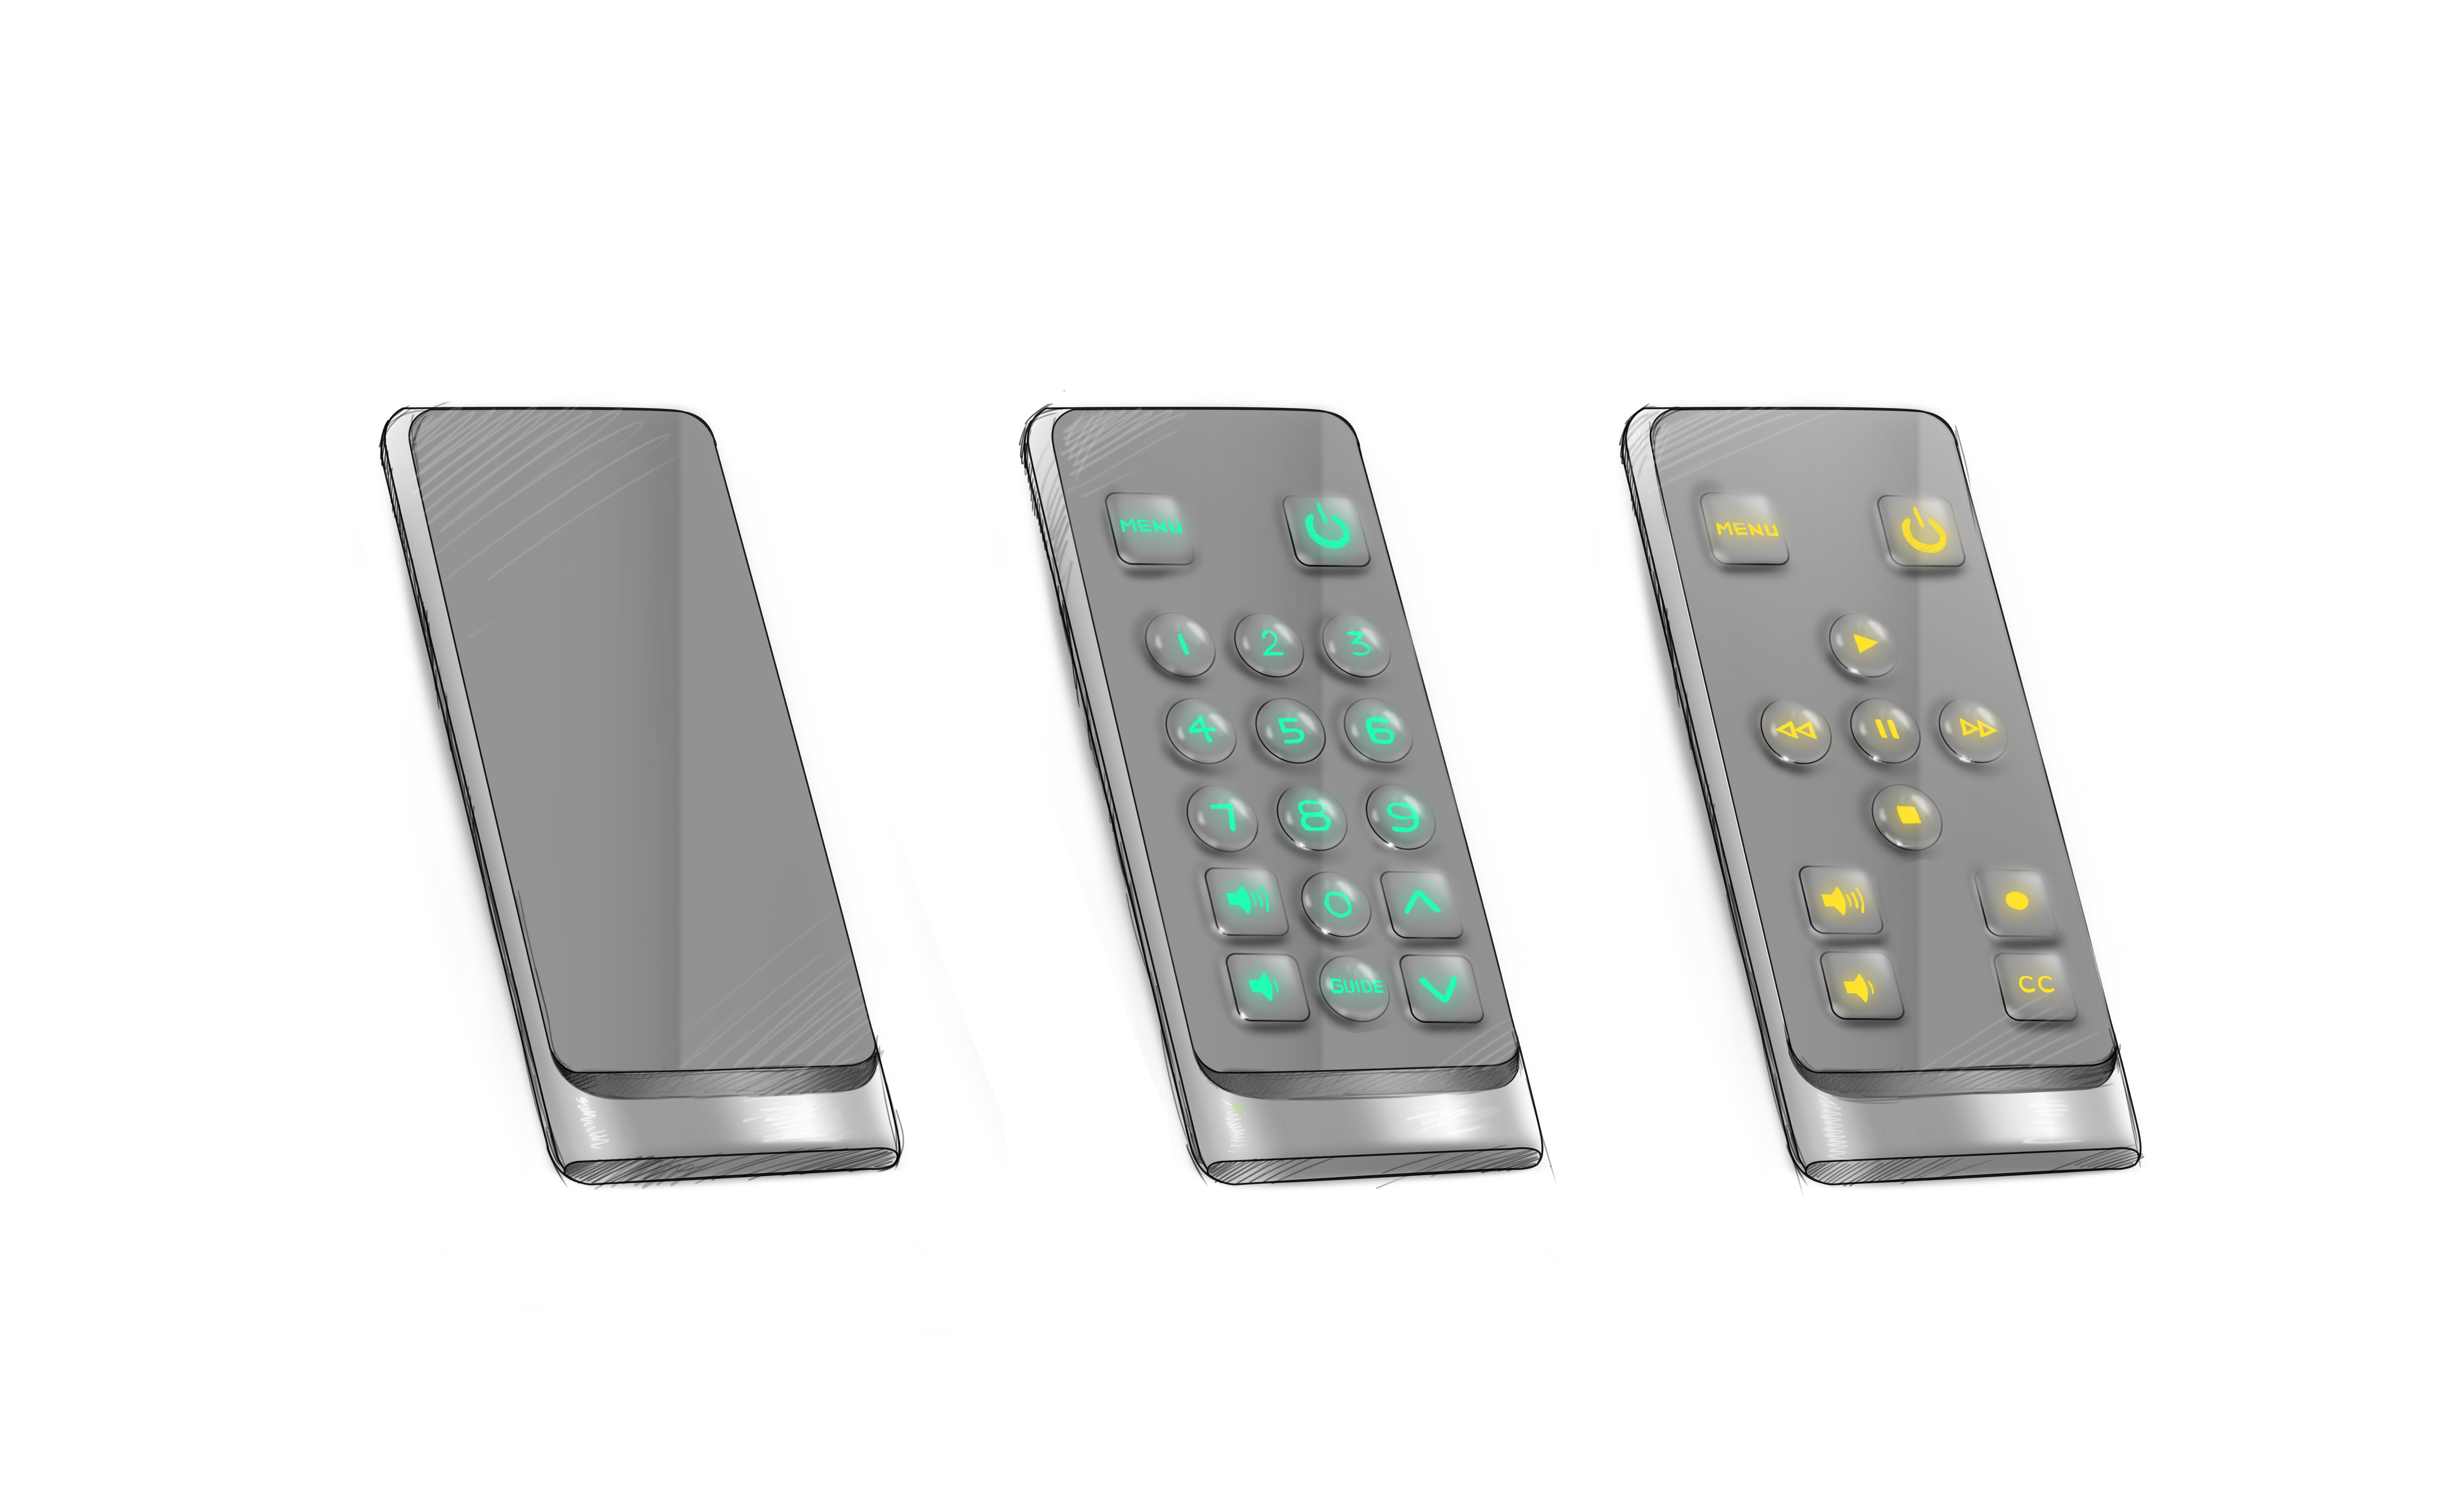
\includegraphics[width=6in]{buttons.jpg}
\caption{A simple representation demonstrating the idea of different subsets of buttons rising up on the same surface at different times.}
\label{buttons}
\end{figure}

In instances when less options are available to the user, less buttons should rise up from the screen. Similarly, when more options are available to the user, more buttons should rise up from the screen. This design aspect should provide more clarity with respect to control flow and what the user is capable of doing at any moment.

\subsection{Auditory Feedback}
The design of this interface was created in such a way that the tactile aspects are intended to operate in conjunction with other technologies that provide auditory feedback. This feedback can inform the user of \textit{what} is at the location on the screen whereas the tactile buttons and grid helps the user know \textit{where} it is.


\section{Usage Scenarios}
There exist several usage scenarios for this interface design. Sighted users employ vision to tell the user what and where to touch, but this interface lacks accessibility for IBSVI because it lacks physical landmarks and tangible buttons. A typical solution is to provide voice over to provide this information, but there is nothing to guide IBSVI to that location in the first place, and there are no landmarks other than dead-reckoning and pure spatial memory to support navigation for the IBSVI. For example, the Apple operating system, iOS, has VoiceOver function, and the Android OS has a Talkbalk function. iOS VoiceOver reads aloud the icon, the user should double tap on that location without the benefit of vision to ensure that the finger does not stray from the touch point. 

The problem with such accessibility modes is that the user can develop a spatial mental model for the interface or screed only through dead reckoning to find VoiceOver locations, in the absence of any landmark other than the boundary of the device. The optional tactile grid as well as the three-dimensional buttons that appear with this design solves this problem. The additional tactile feedback and physical landmarks can guide IBSVI to interact efficiently and effectively with the touch device and its voice over functionality.

Another use case for this interface pertains specifically to the ``intelligent'' tactile buttons. Users often may get overwhelmed by the number of options that are always available to them. It also may be frustrating for users to try to perform a task and not be able to. To examine a specific example, let's say that the user cannot take any more photos on their phone since they are out of memory. In this case, the interface would not even raise the button used to capture photos. This is a good indicator to the user that they need to perform some kind of an action before proceeding.

\section{Rationale}
This layout is designed so that IBSVI so that they can engage their spatial cognition, perception and sensing resources while interacting with touch screens. The design will only enable the grid-like system on-command so to not distract or annoy those who do not benefit from it.

Feedback. In design, it is important to show the effect of an action. Without feedback, one is always wondering whether anything has hap- pened. Maybe the button wasn't pushed hard enough; maybe the machine has stopped working; maybe it is doing the wrong thing. Without feed- back, we turn equipment off at improper times or restart unnecessarily, losing all our recent work. Or we repeat the command and end up having the operation done twice, often to our detriment. Feedback is critical (the design of everyday things).

In the good old days of the telephone, before the American tele- phone system was divided among competing companies, before tele- phones were fancy and had so many features, telephones were de- signed with much more care and concern for the user. Designers at the Bell Telephone Laboratories worried a lot about feedback. The push buttons were designed to give an appropriate feel—tactile feedback. When a button was pushed, a tone was fed back into the earpiece so the user could tell that the button had been properly pushed. When the phone call was being connected, clicks, tones, and other noises gave the user feedback about the progress of the call. And the speaker's voice was always fed back to the earpiece in a carefully controlled amount, because the auditory feedback (called "sidetone") helped the person regulate how loudly to talk. All this has changed. We now have tele- phones that are much more powerful and often cheaper than those that existed just a few years ago—more function for less money. To be fair, these new designs are pushing hard on the paradox of technology: added functionality generally comes along at the price of added com- plexity. But that does not justify backward progress. 
Why are the modern telephone systems so difficult to learn and to use? Basically, the problem is that the systems have more features and less feedback. Suppose all telephones had a small display screen, not unlike the ones on small, inexpensive calculators. The display could be used to present, upon the push of a button, a brief menu of all the features of the telephone, one by one. When the desired one was encountered, the user would push another button to indicate that it should be invoked. If further action was required, the display could tell the person what to do. The display could even be auditory, with speech instead of a visual display. Only two buttons need be added to the 
telephone: one to change the display, one to accept the option on display. Of course, the telephone would be slightly more expensive. The tradeoff is cost versus usability.

Usability research evaluating touchscreen efficacy for both IBSVI and sighted users
still needs to be covered in the literature. I completely agree that the lack of accessibility
for IBSVI is a major issue with touchscreen devices. However, providing more tactile
feedback can increase usability not just for IBSVI, but also for sighted users. In Donald
Norman’s book, The Design of Everyday Things, Norman touches on this principle of
feedback. Norman describes how telephones in the past “were designed with much
more care and concern for the user” as “the push buttons were designed to give an
appropriate feel—tactile feedback.” [20] Norman asserts that modern telephone systems
are “so difficult to use” since they have “more features and less feedback.” [20] As tactile
feedback is significant for IBSVI and sighted users alike, research should examine how
both groups of users respond to proposed solutions. I think that this could possibly
lead to a solution that becomes more widely accepted.


\section{Usability Metric ``Forecast''}
Predict to see an increase in learnability for sighted users and IBSVI alike. Should be more efficient for IBSVI but may be slightly less efficient for sighted users. They can no longer press a button quite as easily. Now that buttons are physical, they will have to lift their finger slightly more and press down slightly harder. This should not take any major hits with efficiency. Rate of errors should be less for both parties.
\clearpage


\bibliography{mybib}{}
\bibliographystyle{plain}
\end{document}

\end{document}
	